\documentclass[11pt]{article}
\usepackage[margin=1in]{geometry}
\usepackage{amsmath,amssymb,amsthm}
\usepackage{booktabs,graphicx,caption}
\usepackage[hidelinks]{hyperref}
\usepackage{natbib}
\newtheorem{proposition}{Proposition}
\newcommand{\e}{\varepsilon}
\setlength{\parskip}{4pt}

\title{AI Capital versus Regular Capital:\\
Output, Real Interest Rates, Wages and the Labor Share,\\ and the Role of the Saving Model}
\author{Research note (draft)}
\date{October 2026}

\begin{document}
\maketitle

\begin{abstract}
\noindent How does technical progress in AI capital move output, the real interest rate,
the real wage and the labor share, compared with progress in regular capital? Regular capital
and labor form a Cobb-Douglas bundle, and AI capital substitutes for that bundle.
Progress is either disembodied (in the production function) or embodied (a lower price
of new capital in the accumulation equation). It arrives as a surprise jump, as an
S-curve complete by year 10, or half and half. Every shock is a one-time level shift
that raises long-run output by the same 10 percent. Under the standard Ramsey saving
model, the long run is in closed form. AI progress raises the wage by
$1/[1+(1-a)(\e-1)]$ of the output gain (74 percent here) and lowers the labor share,
while regular-capital progress raises the wage one-for-one. In the short run, the
real-rate response depends much more on whether progress is embodied and on its timing than on
substitutability. Substitutability matters for $r$ only after a surprise
disembodied jump. That conclusion depends on the Ramsey assumption of perfectly
elastic long-run capital supply. Under Solow (fixed saving), Diamond OLG,
annual-frequency OLG and perpetual-youth saving, regular-capital progress still leaves
long-run $r$ unchanged. AI progress, however, changes long-run $r$ exactly when
$\e\neq1$. For $\e=1.5$, $r$ rises by 1.1 percentage points under Solow, 0.4 under Diamond, 0.1 under
the annual OLG and essentially zero under Ramsey.
\end{abstract}

\section{Questions and main findings}

The note asks three questions:
\begin{enumerate}
\item Do AI and regular-capital progress affect the interest rate, wages and the labor
share differently, holding the long-run output gain fixed?
\item How much of the difference comes from AI's substitutability for labor and capital?
\item How much depends on the saving model, given that the Ramsey Euler equation makes
long-run capital supply perfectly elastic?
\end{enumerate}
Main findings:
\begin{itemize}
\item \emph{Wages and the labor share} differ sharply between AI and regular-capital
progress. The difference comes from substitutability, and it holds in every saving model.
\item \emph{The real interest rate} under Ramsey depends mainly on whether progress is
embodied and on its timing. Substitutability matters little, except after surprise
disembodied jumps.
\item \emph{Long-run interest rates} respond to AI progress, and through substitutability,
once saving is not perfectly elastic. Regular-capital progress inside the Cobb-Douglas
bundle never moves long-run $r$.
\end{itemize}

\section{Model}

Notation follows \citet{kiley2000}. Production is
\begin{equation*}
X=(\Gamma_KK)^a(ZN)^{1-a},\qquad
Y=\Big[\omega^{1/\e}X^{\frac{\e-1}{\e}}+(1-\omega)^{1/\e}(\Gamma_AA)^{\frac{\e-1}{\e}}\Big]^{\frac{\e}{\e-1}},
\qquad \e=1.5\ \text{(baseline)}.
\end{equation*}
Capital $j\in\{K,A\}$ is measured in efficiency units: $K_j'=(1-d_j)K_j+I_j/P_j$.
\emph{Disembodied} progress raises $\Gamma_j$, which improves installed capital.
\emph{Embodied} progress lowers $P_j$, which improves only new investment. Hours are
fixed and trend growth is $g=1.5$ percent.

\paragraph{Experiments.} Each is a one-time, permanent level shift in $\Gamma_j$ or $1/P_j$,
announced at $t=0$, with three timings:
\begin{itemize}
\item a \emph{jump} at $t=0$;
\item an \emph{S-curve}, $S_t=\tfrac12[1-\cos(\pi t/10)]$, which starts at $t=0$ and is complete by year 10;
\item \emph{half/half}: half the log improvement as a jump, half along the S-curve.
\end{itemize}
Elasticities are the same in every experiment. Each shock is scaled \emph{within each
model} so that long-run output, relative to the pre-shock path, rises by 10 percent.

\paragraph{Calibration.} $a=0.282$, $d_K=0.066$, initial $r=7.5$ percent, initial AI
income share 3 percent, initial labor share 69.6 percent. Two accumulation settings are
used:
\begin{itemize}
\item[(A)] $d_A=0.20$, with the adjustment costs of \citet{kiley2004},
$P_j\tfrac{c_j}{2}(i_j-x_j)^2K_j$, where $i_j=I_j/(P_jK_j)$, $x_j=g+d_j$ and $c_j=1/x_j$, so that
both stocks have a unit elasticity of investment to $Q$;
\item[(B)] $d_A=d_K=0.066$ and no adjustment costs. This isolates substitutability from
differences in depreciation and adjustment costs.
\end{itemize}

\section{Closed-form long run}

\begin{proposition}[Balanced growth path]\label{prop:bgp}
With constant technology levels and real rate $r$, $Q_j=P_j$ and $u_j=r+d_j$. With
$\lambda_j=P_ju_j/\Gamma_j$,
\begin{gather*}
s_A=(1-\omega)\lambda_A^{1-\e},\quad
\text{labor share}=(1-a)(1-s_A),\quad
P_X=\Big(\frac{1-s_A}{\omega}\Big)^{\frac1{1-\e}},\\
\ln\frac WZ=\frac{\ln P_X}{1-a}-\frac{a}{1-a}\ln\lambda_K+\text{const},\qquad
\ln\frac YZ=\ln\frac WZ-\ln(1-s_A)+\text{const}.
\end{gather*}
\end{proposition}

\begin{proposition}[Same output gain $\gamma_Y$, given $r$]\label{prop:lr}
Disembodied and embodied progress have the same long-run effects ($\ln\Gamma_j=-\ln P_j$).
\emph{Regular capital}: $\ln(\Gamma_K/P_K)=\frac{1-a}{a}\gamma_Y$, $\Delta\ln W=\gamma_Y$, and the labor share is unchanged.
\emph{AI}: $\Delta\ln W=\dfrac{\gamma_Y}{1+(1-a)(\e-1)}$ and
$\Delta\ln(\text{labor share})=-\dfrac{(1-a)(\e-1)}{1+(1-a)(\e-1)}\gamma_Y$.
\end{proposition}
Under Ramsey, $r$ is pinned at $(1+g)/B-1$, so Proposition~\ref{prop:lr} gives the long run
directly. For $\gamma_Y=10$ percent, regular-capital technology rises 29 percent and AI
technology 3.4-fold. The wage rises 10.0 percent (regular capital) or 7.4 percent (AI), and
under AI progress the labor share falls from 69.6 to 67.8 percent.

\section{Dynamics under Ramsey}

\subsection{Setting A: AI depreciates faster and both stocks face adjustment costs}

\begin{figure}[h]\centering
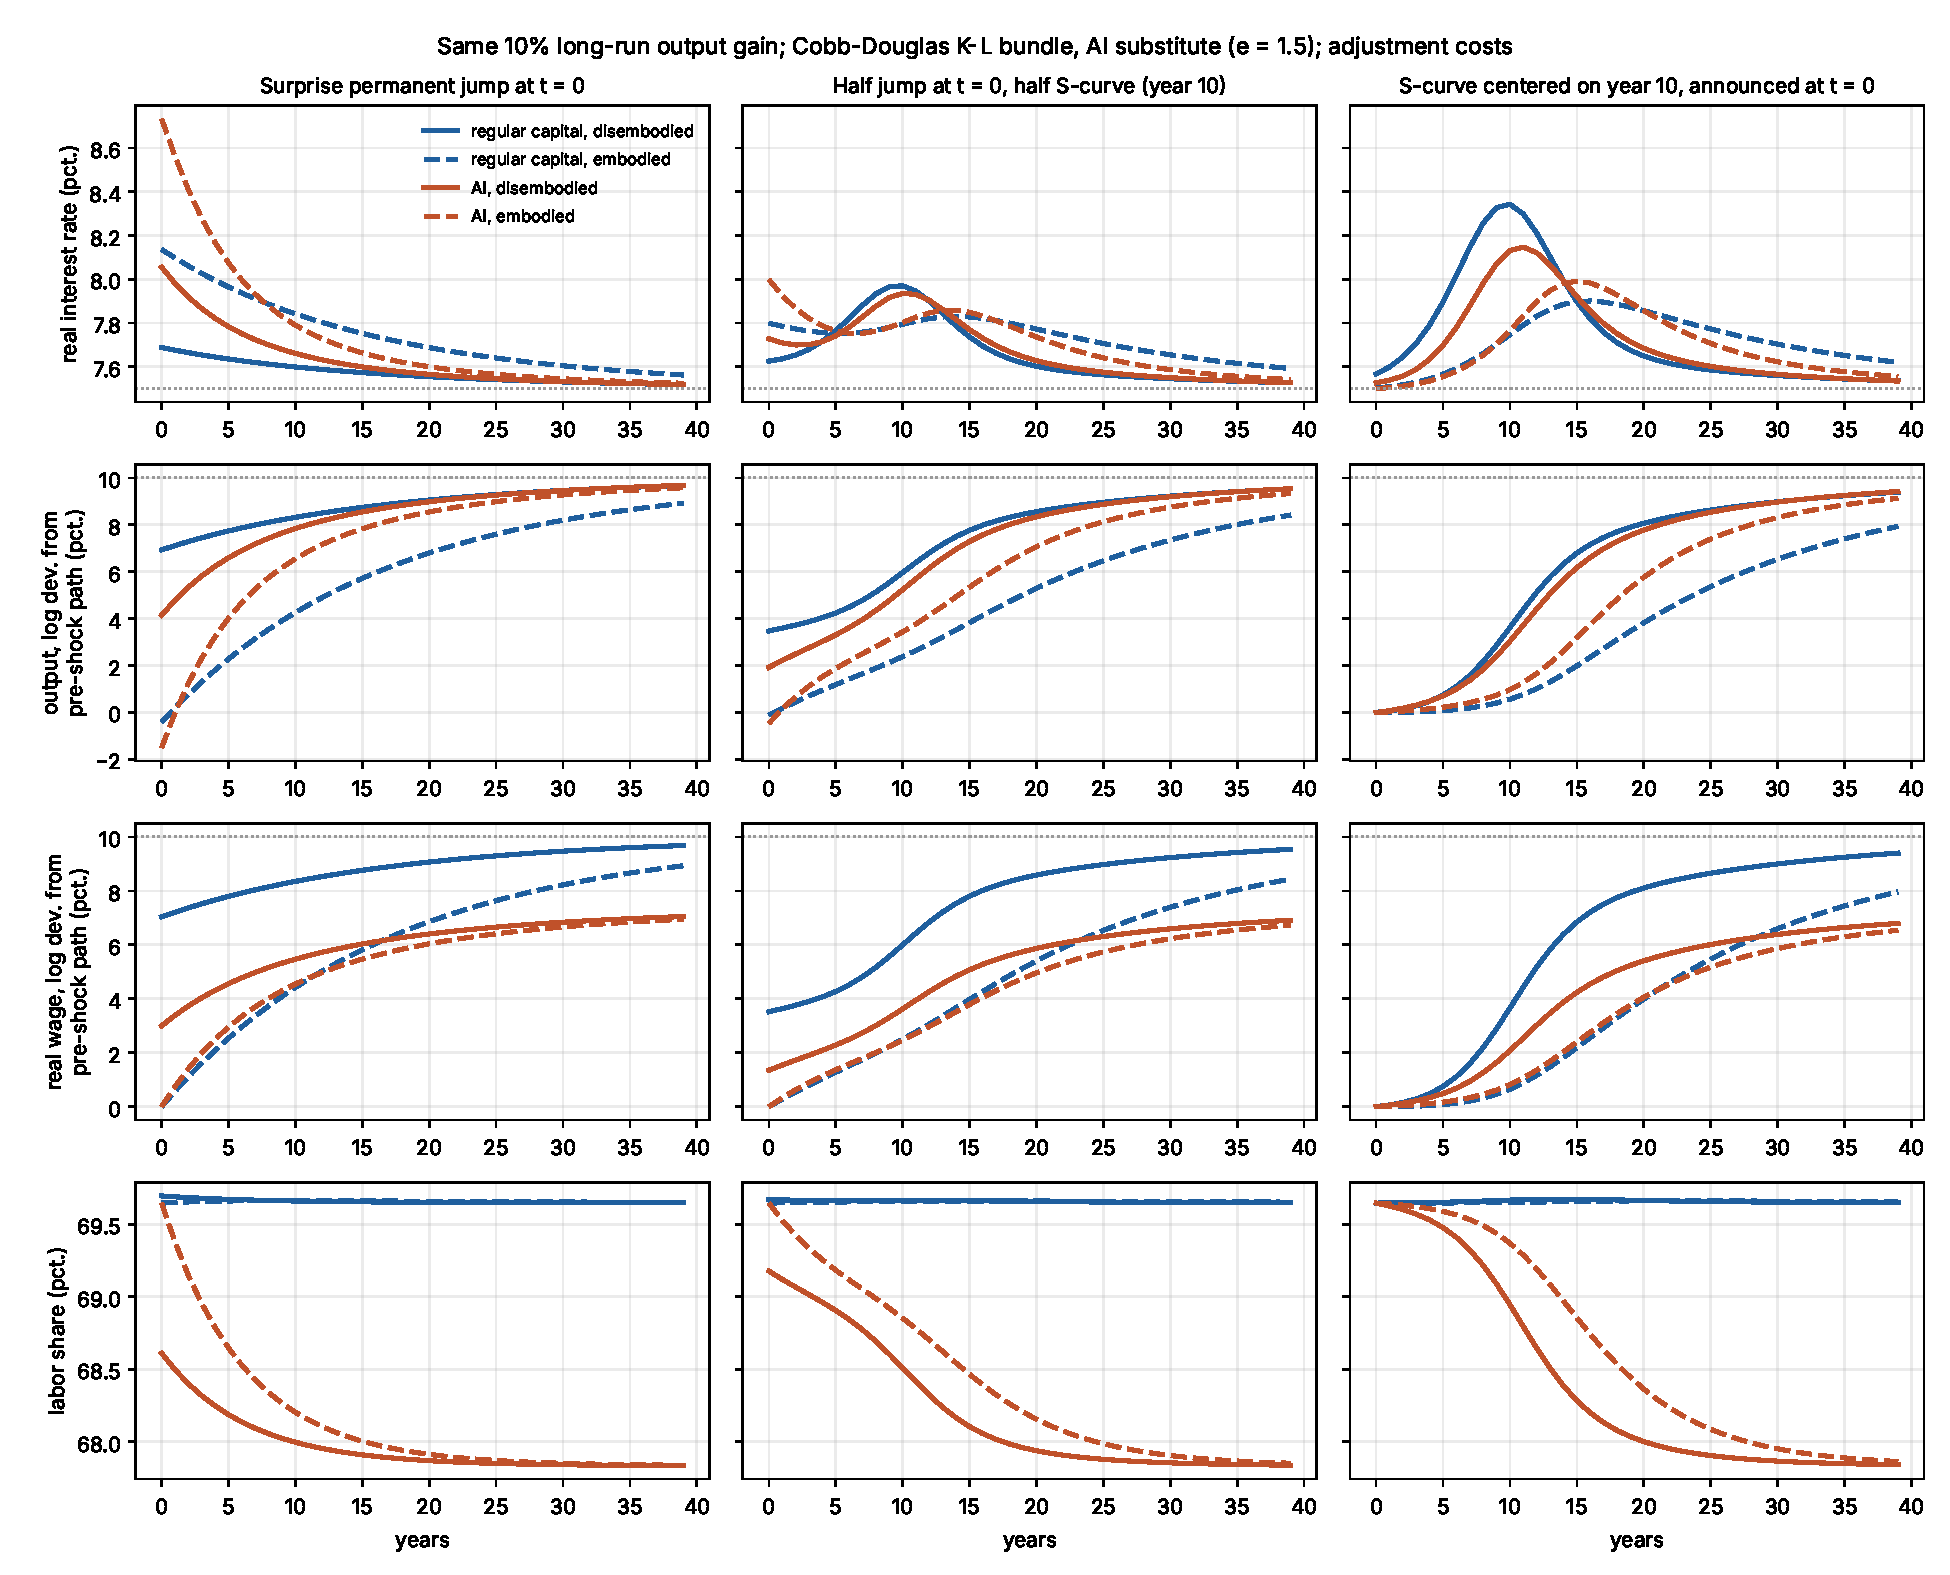
\includegraphics[width=\textwidth]{figures/fig_capital_cases.pdf}
\caption{Setting A ($d_A=0.20$, adjustment costs). Same 10\% long-run output gain.}\label{fig:A}
\end{figure}

\begin{table}[h]\centering\scriptsize
\caption{Setting A. $r_1$ is the rate between years 0 and 1. Output and wages are log deviations (percent) from the pre-shock path.}\label{tab:A}
\begin{tabular}{llcccccccccc}\toprule
 & & \multicolumn{3}{c}{real rate (pct.)} & \multicolumn{3}{c}{output, $\ln Y$ (pct.)} & \multicolumn{3}{c}{real wage, $\ln W$ (pct.)} & labor share\\
\cmidrule(lr){3-5}\cmidrule(lr){6-8}\cmidrule(lr){9-11}\cmidrule(lr){12-12}
 & & $r_1$ & peak & year & $t{=}0$ & $t{=}10$ & $t{=}20$ & $t{=}0$ & $t{=}10$ & $t{=}20$ & $t{=}10$ (pct.)\\\midrule
Jump & Regular, disemb. & 7.69 & 7.69 & 0 & 6.9 & 8.3 & 9.1 & 7.0 & 8.4 & 9.1 & 69.7\\
 & Regular, emb. & 8.14 & 8.14 & 0 & -0.4 & 4.3 & 6.8 & 0.0 & 4.4 & 6.9 & 69.7\\
 & AI, disemb. & 8.05 & 8.05 & 0 & 4.1 & 7.8 & 9.0 & 3.0 & 5.5 & 6.4 & 68.0\\
 & AI, emb. & 8.73 & 8.73 & 0 & -1.5 & 6.6 & 8.6 & 0.0 & 4.5 & 6.0 & 68.2\\
\midrule
Half/half & Regular, disemb. & 7.69 & 8.20 & 5 & 3.5 & 8.0 & 8.9 & 3.5 & 8.0 & 8.9 & 69.7\\
 & Regular, emb. & 7.80 & 7.93 & 9 & -0.1 & 3.1 & 6.2 & 0.0 & 3.3 & 6.2 & 69.7\\
 & AI, disemb. & 7.76 & 8.17 & 5 & 1.9 & 7.4 & 8.8 & 1.4 & 5.1 & 6.2 & 68.0\\
 & AI, emb. & 7.99 & 8.04 & 8 & -0.5 & 4.8 & 8.1 & 0.0 & 3.5 & 5.7 & 68.5\\
\midrule
S-curve & Regular, disemb. & 7.69 & 8.76 & 5 & 0.0 & 7.6 & 8.7 & 0.0 & 7.7 & 8.7 & 69.7\\
 & Regular, emb. & 7.51 & 7.99 & 9 & 0.0 & 1.9 & 5.5 & 0.0 & 2.2 & 5.6 & 69.7\\
 & AI, disemb. & 7.57 & 8.50 & 6 & -0.1 & 7.0 & 8.6 & 0.0 & 4.8 & 6.1 & 68.1\\
 & AI, emb. & 7.50 & 8.20 & 9 & 0.0 & 3.3 & 7.7 & 0.0 & 2.6 & 5.4 & 68.8\\
\bottomrule\end{tabular}

\end{table}

\begin{itemize}
\item \emph{Real rate.} After a jump, $r$ rises most for embodied AI (8.7 percent), then
embodied regular capital (8.1), disembodied AI (8.05) and disembodied regular capital
(7.7). Along the S-curve it peaks earlier and higher under disembodied progress: 8.8
(regular) and 8.5 (AI) around years 5--6, against 8.0 and 8.2 around year 9 under embodied
progress. The half/half case lies between the two.
\item \emph{Output.} Disembodied progress raises output on impact (6.9 percent regular,
4.1 AI). An embodied jump briefly \emph{lowers} net output (by 0.4 and 1.5 percent), because
the investment boom absorbs resources in adjustment costs. AI output catches up quickly
because AI capital turns over fast.
\item \emph{Wages and the labor share.} AI wages lag AI output, because the AI share rises. The
labor share moves only under AI progress.
\end{itemize}

\subsection{Setting B: equal depreciation and no adjustment costs}

\begin{figure}[h]\centering
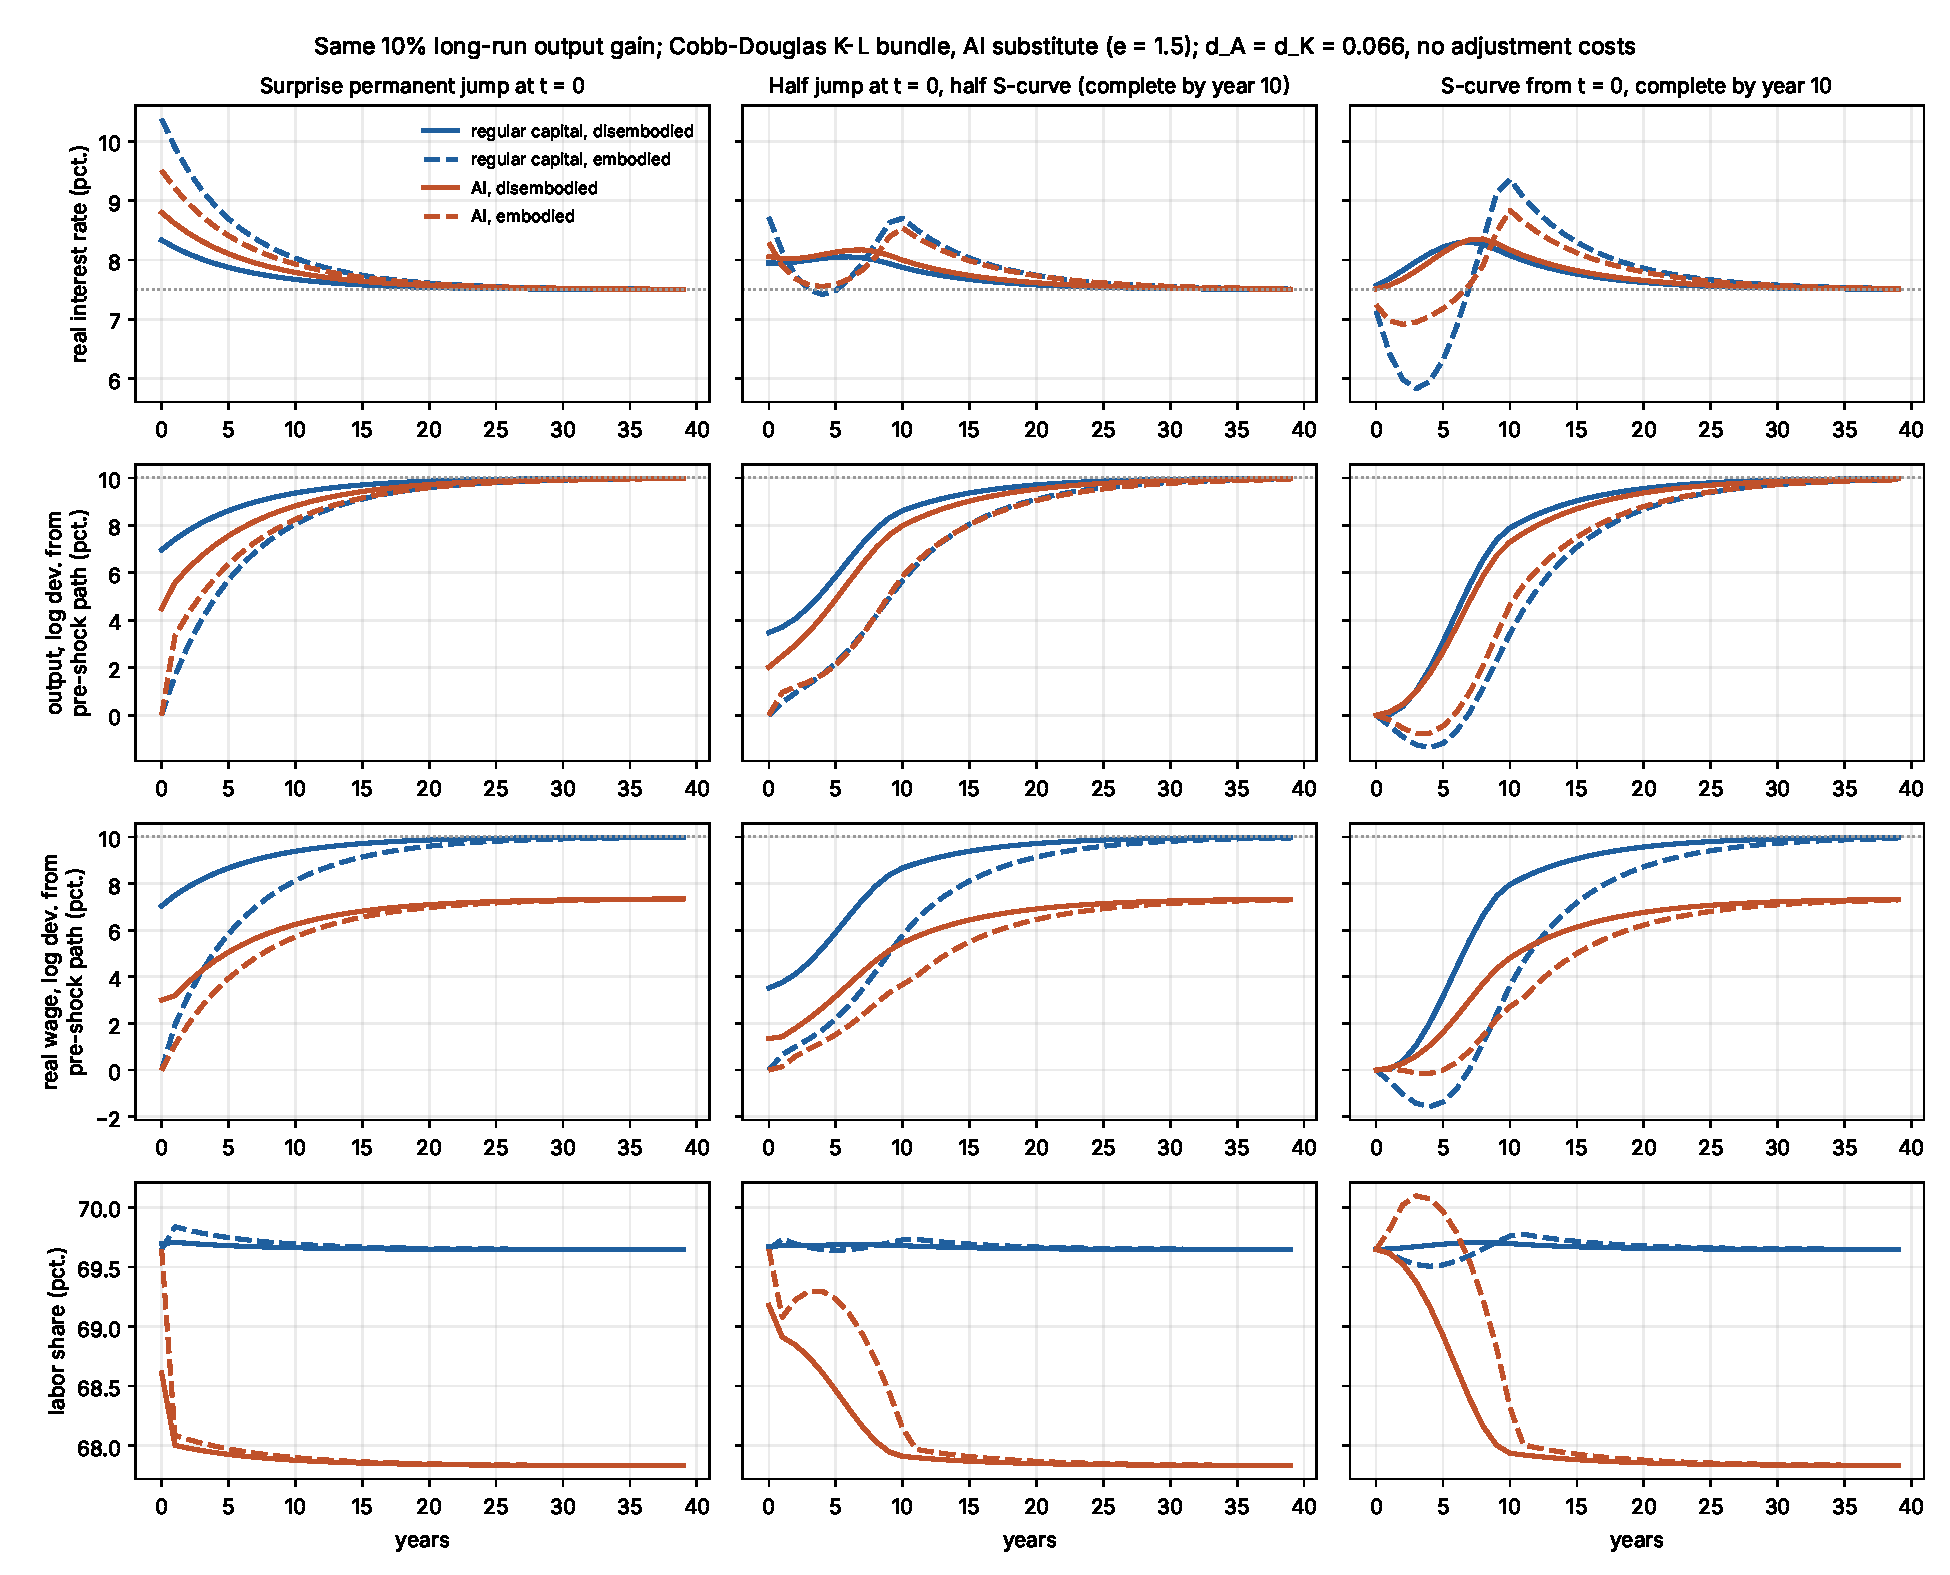
\includegraphics[width=\textwidth]{figures/fig_capital_cases_eqd_noadj.pdf}
\caption{Setting B ($d_A=d_K=0.066$, no adjustment costs).}\label{fig:B}
\end{figure}

\begin{table}[h]\centering\scriptsize
\caption{Setting B. Columns as in Table~\ref{tab:A}.}\label{tab:B}
\begin{tabular}{llcccccccccc}\toprule
 & & \multicolumn{3}{c}{real rate (pct.)} & \multicolumn{3}{c}{output, $\ln Y$ (pct.)} & \multicolumn{3}{c}{real wage, $\ln W$ (pct.)} & labor share\\
\cmidrule(lr){3-5}\cmidrule(lr){6-8}\cmidrule(lr){9-11}\cmidrule(lr){12-12}
 & & $r_1$ & peak & year & $t{=}0$ & $t{=}10$ & $t{=}20$ & $t{=}0$ & $t{=}10$ & $t{=}20$ & $t{=}10$ (pct.)\\\midrule
Jump & Regular, disemb. & 8.33 & 8.33 & 0 & 7.0 & 9.4 & 9.9 & 7.0 & 9.4 & 9.9 & 69.7\\
 & Regular, emb. & 10.38 & 10.38 & 0 & 0.0 & 8.1 & 9.6 & 0.0 & 8.1 & 9.6 & 69.7\\
 & AI, disemb. & 8.80 & 8.80 & 0 & 4.5 & 8.8 & 9.7 & 3.0 & 6.2 & 7.1 & 67.9\\
 & AI, emb. & 9.51 & 9.51 & 0 & 0.0 & 8.3 & 9.6 & 0.0 & 5.7 & 7.0 & 67.9\\
\midrule
Half/half & Regular, disemb. & 7.95 & 8.05 & 6 & 3.5 & 8.6 & 9.7 & 3.5 & 8.7 & 9.7 & 69.7\\
 & Regular, emb. & 8.72 & 8.72 & 0 & 0.0 & 5.7 & 9.1 & 0.0 & 5.8 & 9.1 & 69.7\\
 & AI, disemb. & 8.06 & 8.17 & 7 & 2.0 & 8.0 & 9.5 & 1.4 & 5.5 & 6.9 & 67.9\\
 & AI, emb. & 8.29 & 8.53 & 10 & 0.0 & 5.9 & 9.0 & 0.0 & 3.7 & 6.5 & 68.1\\
\midrule
S-curve & Regular, disemb. & 7.57 & 8.30 & 7 & 0.0 & 7.9 & 9.6 & 0.0 & 8.0 & 9.6 & 69.7\\
 & Regular, emb. & 7.14 & 9.36 & 10 & 0.0 & 3.4 & 8.7 & 0.0 & 3.6 & 8.7 & 69.8\\
 & AI, disemb. & 7.51 & 8.35 & 8 & 0.0 & 7.3 & 9.4 & 0.0 & 4.8 & 6.8 & 67.9\\
 & AI, emb. & 7.24 & 8.83 & 10 & 0.0 & 4.6 & 8.8 & 0.0 & 2.7 & 6.2 & 68.3\\
\bottomrule\end{tabular}

\end{table}

Without adjustment costs, investment responds faster and $r$ moves more.
\begin{itemize}
\item \emph{Embodied regular-capital progress} has the largest impact effect, 10.4
percent after a jump. Regular capital is a much larger stock than AI, so it requires
the largest investment swing.
\item \emph{An anticipated embodied S-curve} produces a two-phase response. Firms wait
for cheaper capital, so $r$ first \emph{falls} (to 5.8 percent for regular capital and
6.9 for AI) and output and wages dip. Then an investment boom pushes $r$ to 9.4 (regular)
or 8.8 percent (AI) at year 10.
\item \emph{Capital adjusts within a year}, so after an AI jump the labor share falls
almost entirely by year 1.
\end{itemize}

\subsection{How much does substitutability matter for $r$?}

Table~\ref{tab:eps} varies only AI's elasticity in Setting B, from 0.75 (near the
complements limit, where a 10 percent output gain needs a roughly 150-fold improvement
in AI technology) to 2. Comparing AI and regular capital directly confounds
substitutability with AI's small initial share. This experiment does not.

\begin{table}[h]\centering\scriptsize
\caption{Ramsey, Setting B, AI progress, varying $\e$. ``40-yr excess'' is $\sum_{t<40}[\ln(1+r_{t+1})-\ln 1.075]$ in percentage points.}\label{tab:eps}
\begin{tabular}{lcccccccc}\toprule
 & \multicolumn{2}{c}{jump, disemb.} & \multicolumn{2}{c}{jump, emb.} & S-curve, disemb. & S-curve, emb. & \multicolumn{2}{c}{long run}\\
\cmidrule(lr){2-3}\cmidrule(lr){4-5}\cmidrule(lr){6-6}\cmidrule(lr){7-7}\cmidrule(lr){8-9}
$\e$ (AI) & $r_1$ & 40-yr excess & $r_1$ & 40-yr excess & peak & trough/peak & $\Delta\ln W$ & labor share\\\midrule
0.75 & 7.96 & 2.8 & 9.10 & 9.3 & 8.26 & 6.74/8.54 & 12.2 & 71.2\\
1 & 8.36 & 5.4 & 9.38 & 11.3 & 8.31 & 6.90/8.79 & 10.0 & 69.6\\
1.5 & 8.80 & 8.6 & 9.51 & 13.0 & 8.35 & 6.91/8.83 & 7.4 & 67.8\\
2 & 8.95 & 10.2 & 9.46 & 13.5 & 8.36 & 6.91/8.78 & 5.8 & 66.8\\
\bottomrule\end{tabular}

\end{table}

\begin{itemize}
\item \emph{Along an S-curve and for embodied shocks}, $\e$ barely moves $r$. Peaks and
troughs change by 0.1--0.4 points across the whole range.
\item \emph{After a surprise disembodied jump}, $\e$ matters. $r_1$ rises from 8.0 to 9.0
percent, and the 40-year cumulative excess return from 2.8 to 10.2 points. With higher $\e$,
less of the output gain arrives on impact, more must come from accumulation, and expected
consumption growth is higher.
\item \emph{Wages and the labor share} are highly sensitive to $\e$. The long-run wage gain
falls from 12.2 to 5.8 percent, and the labor share from 71.2 to 66.8 percent.
\end{itemize}
At $\e=1$, disembodied AI and disembodied regular-capital progress produce identical
paths, as theory implies.

\section{The saving model}

\paragraph{Why Ramsey pins $r$.} With an infinitely lived household, the steady-state
Euler equation fixes $1+r=(1+g)/B$, so long-run capital supply is perfectly
elastic. Saving adjusts to whatever is needed to deliver that rate, and no level shift
in technology can move long-run $r$. The closed-form CES-pairing models of the
companion note have constant saving \emph{rates}, but they too pin $r$ by $B$ and $g$.

\paragraph{Alternatives} (all with Setting B, $\e=1.5$ unless noted, and recalibrated to the same initial path):
\begin{itemize}
\item \emph{Solow}: a fixed gross saving rate $s$.
\item \emph{Perpetual youth} \citep{blanchard1985,yaari1965}: death probability $p=0.025$
(a 40-year horizon), annuities, log utility and flat labor income, so that
$C=[1-B(1-p)](A+H)$, where $H$ is human wealth discounted at $(1+r)/(1-p)$. With $p=0$ this is Ramsey.
\item \emph{Annual OLG}: 60 cohorts (ages 20--79) who work for 45 years with flat earnings, log
utility and no bequests. Cohorts alive at $t=0$ hold their steady-state wealth,
revalued by the shock.
\item \emph{Diamond OLG} \citep{diamond1965}: two 30-year periods, with the young saving
$B_L/(1+B_L)$ of wages. Long run only.
\end{itemize}

\begin{proposition}[Long-run interest rate]\label{prop:saving}
In every model, the capital share is $1-(1-a)(1-s_A)$ and wealth relative to output is
(capital share)$/(r+d)$. Long-run $r$ solves:
\begin{align*}
\text{Ramsey:}&\quad 1+r=(1+g)/B;\\
\text{Solow:}&\quad (g+d)\,\frac{\text{capital share}}{r+d}=s;\\
\text{Diamond:}&\quad r_L+d_L=(1+g)^L\,\frac{\text{capital share}}{s_y\cdot\text{labor share}};\\
\text{Annual OLG, perpetual youth:}&\quad \text{household wealth}(r)\cdot\text{labor share}=(1+r)\,\frac{\text{capital share}}{r+d},
\end{align*}
with household wealth per unit of labor income in closed form for each (a 60-term sum for the
OLG; a geometric sum for perpetual youth). With a Cobb-Douglas bundle, regular-capital
progress leaves the capital share unchanged at every $r$, so it never changes long-run $r$. AI
progress changes the capital share if and only if $\e\neq1$. It then raises $r$ if $\e>1$ and
lowers it if $\e<1$, in every model where capital supply is not perfectly elastic.
\end{proposition}

\begin{figure}[h]\centering
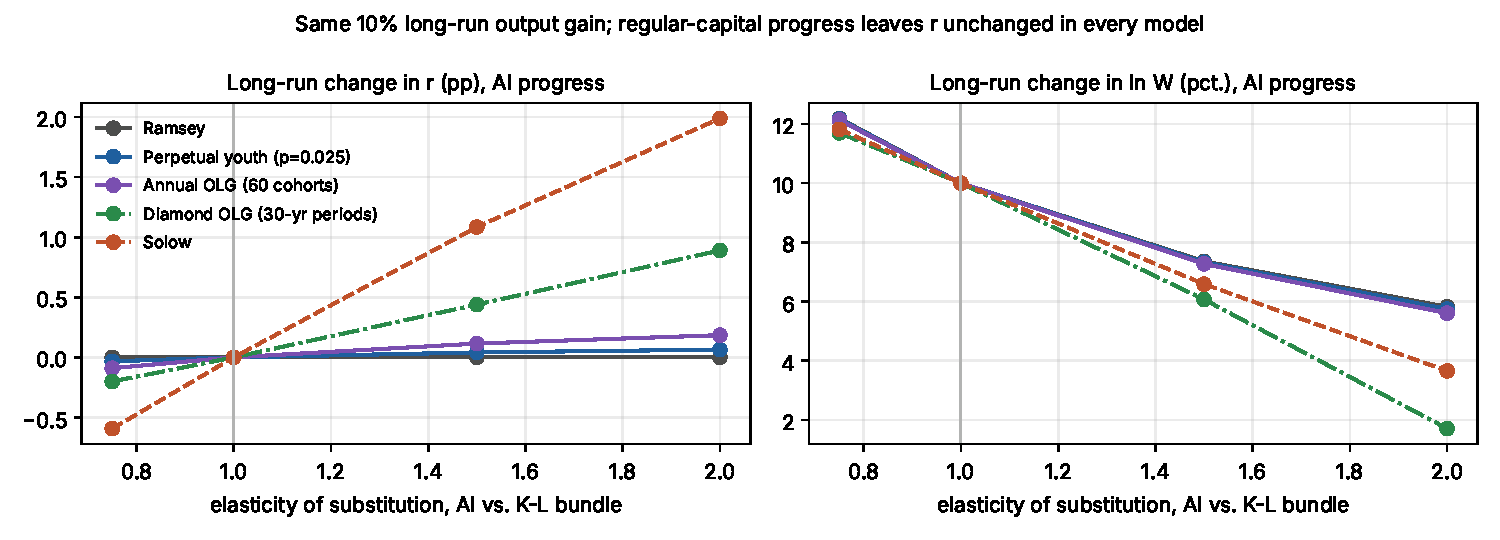
\includegraphics[width=\textwidth]{figures/fig_saving_longrun.pdf}
\caption{Long-run effects of AI progress by saving model and elasticity (same 10\% output gain).}\label{fig:lr}
\end{figure}

\begin{table}[h]\centering\scriptsize
\caption{Long run by saving model. The shock is the log improvement in AI (or regular-capital) technology needed for a 10\% output gain.}\label{tab:lr}
\begin{tabular}{llcccccc}\toprule
$\e$ & saving model & shock (log) & $\Delta r$ (pp) & long-run $r$ & $\Delta\ln W$ & labor share & AI share\\\midrule
0.75 & Ramsey & 5.02 & +0.00 & 7.50 & 12.2 & 71.2 & 0.9\\
0.75 & Perpetual youth (p=0.025) & 4.93 & -0.03 & 7.47 & 12.2 & 71.2 & 0.9\\
0.75 & Solow & 3.56 & -0.59 & 6.91 & 11.8 & 70.9 & 1.2\\
0.75 & Diamond OLG & 3.17 & -0.20 & 7.30 & 11.7 & 70.8 & 1.3\\
\midrule
1 & Ramsey & 2.32 & +0.00 & 7.50 & 10.0 & 69.6 & 3.0\\
1 & Perpetual youth (p=0.025) & 2.32 & +0.00 & 7.50 & 10.0 & 69.6 & 3.0\\
1 & Solow & 2.32 & +0.00 & 7.50 & 10.0 & 69.6 & 3.0\\
1 & Diamond OLG & 2.32 & +0.00 & 7.50 & 10.0 & 69.6 & 3.0\\
\midrule
1.5 & Ramsey & 1.22 & +0.00 & 7.50 & 7.4 & 67.8 & 5.5\\
1.5 & Perpetual youth (p=0.025) & 1.24 & +0.04 & 7.54 & 7.3 & 67.8 & 5.6\\
1.5 & Solow & 1.54 & +1.08 & 8.58 & 6.6 & 67.3 & 6.3\\
1.5 & Diamond OLG & 1.74 & +0.44 & 7.94 & 6.1 & 67.0 & 6.7\\
\midrule
2 & Ramsey & 0.84 & +0.00 & 7.50 & 5.8 & 66.8 & 7.0\\
2 & Perpetual youth (p=0.025) & 0.86 & +0.06 & 7.56 & 5.7 & 66.7 & 7.0\\
2 & Solow & 1.23 & +1.99 & 9.49 & 3.7 & 65.4 & 9.0\\
2 & Diamond OLG & 1.52 & +0.89 & 8.39 & 1.7 & 64.1 & 10.7\\
\midrule
reg. capital & Ramsey & 0.25 & +0.00 & 7.50 & 10.0 & 69.6 & 3.0\\
 & Perpetual youth (p=0.025) & 0.25 & +0.00 & 7.50 & 10.0 & 69.6 & 3.0\\
 & Solow & 0.25 & +0.00 & 7.50 & 10.0 & 69.6 & 3.0\\
 & Diamond OLG & 0.25 & +0.00 & 7.50 & 10.0 & 69.6 & 3.0\\
\bottomrule\end{tabular}

\end{table}

\paragraph{Long-run results (Table~\ref{tab:lr}, Figure~\ref{fig:lr}).}
\begin{itemize}
\item \emph{Regular-capital progress} leaves $r$ unchanged in every model, and wages rise one-for-one with output.
\item \emph{AI progress with $\e=1.5$} raises $r$ by 0 (Ramsey), 0.04 (perpetual youth), 0.11
(annual OLG), 0.44 (Diamond) and 1.08 points (Solow). At $\e=2$ the figures are 0, 0.06, 0.18,
0.89 and 1.99. At $\e=0.75$, $r$ falls in every model except Ramsey.
\item \emph{The less elastic the saving, the more the AI shock must deliver and the less
labor gets.} With the same 10 percent output gain, the required AI improvement rises from
3.4-fold (Ramsey) to 4.7-fold (Solow) and 5.7-fold (Diamond). The wage gain falls from 7.4 to
6.6 and 6.1 percent.
\item \emph{Why the two OLG models differ.} Life-cycle saving in the annual OLG is very
elastic to $r$: $B(1+r)/(1+g)\approx0.995$, so a small rise in $r$ calls forth much more
saving. Its long-run responses are therefore close to Ramsey. In the Diamond model, saving
out of wages makes the proportional change in the 30-year return larger, but compounding
over the period translates it into a moderate change in the annual rate. Perpetual youth
with flat labor income and a 40-year horizon stays close to Ramsey.
\end{itemize}

\begin{figure}[p]\centering
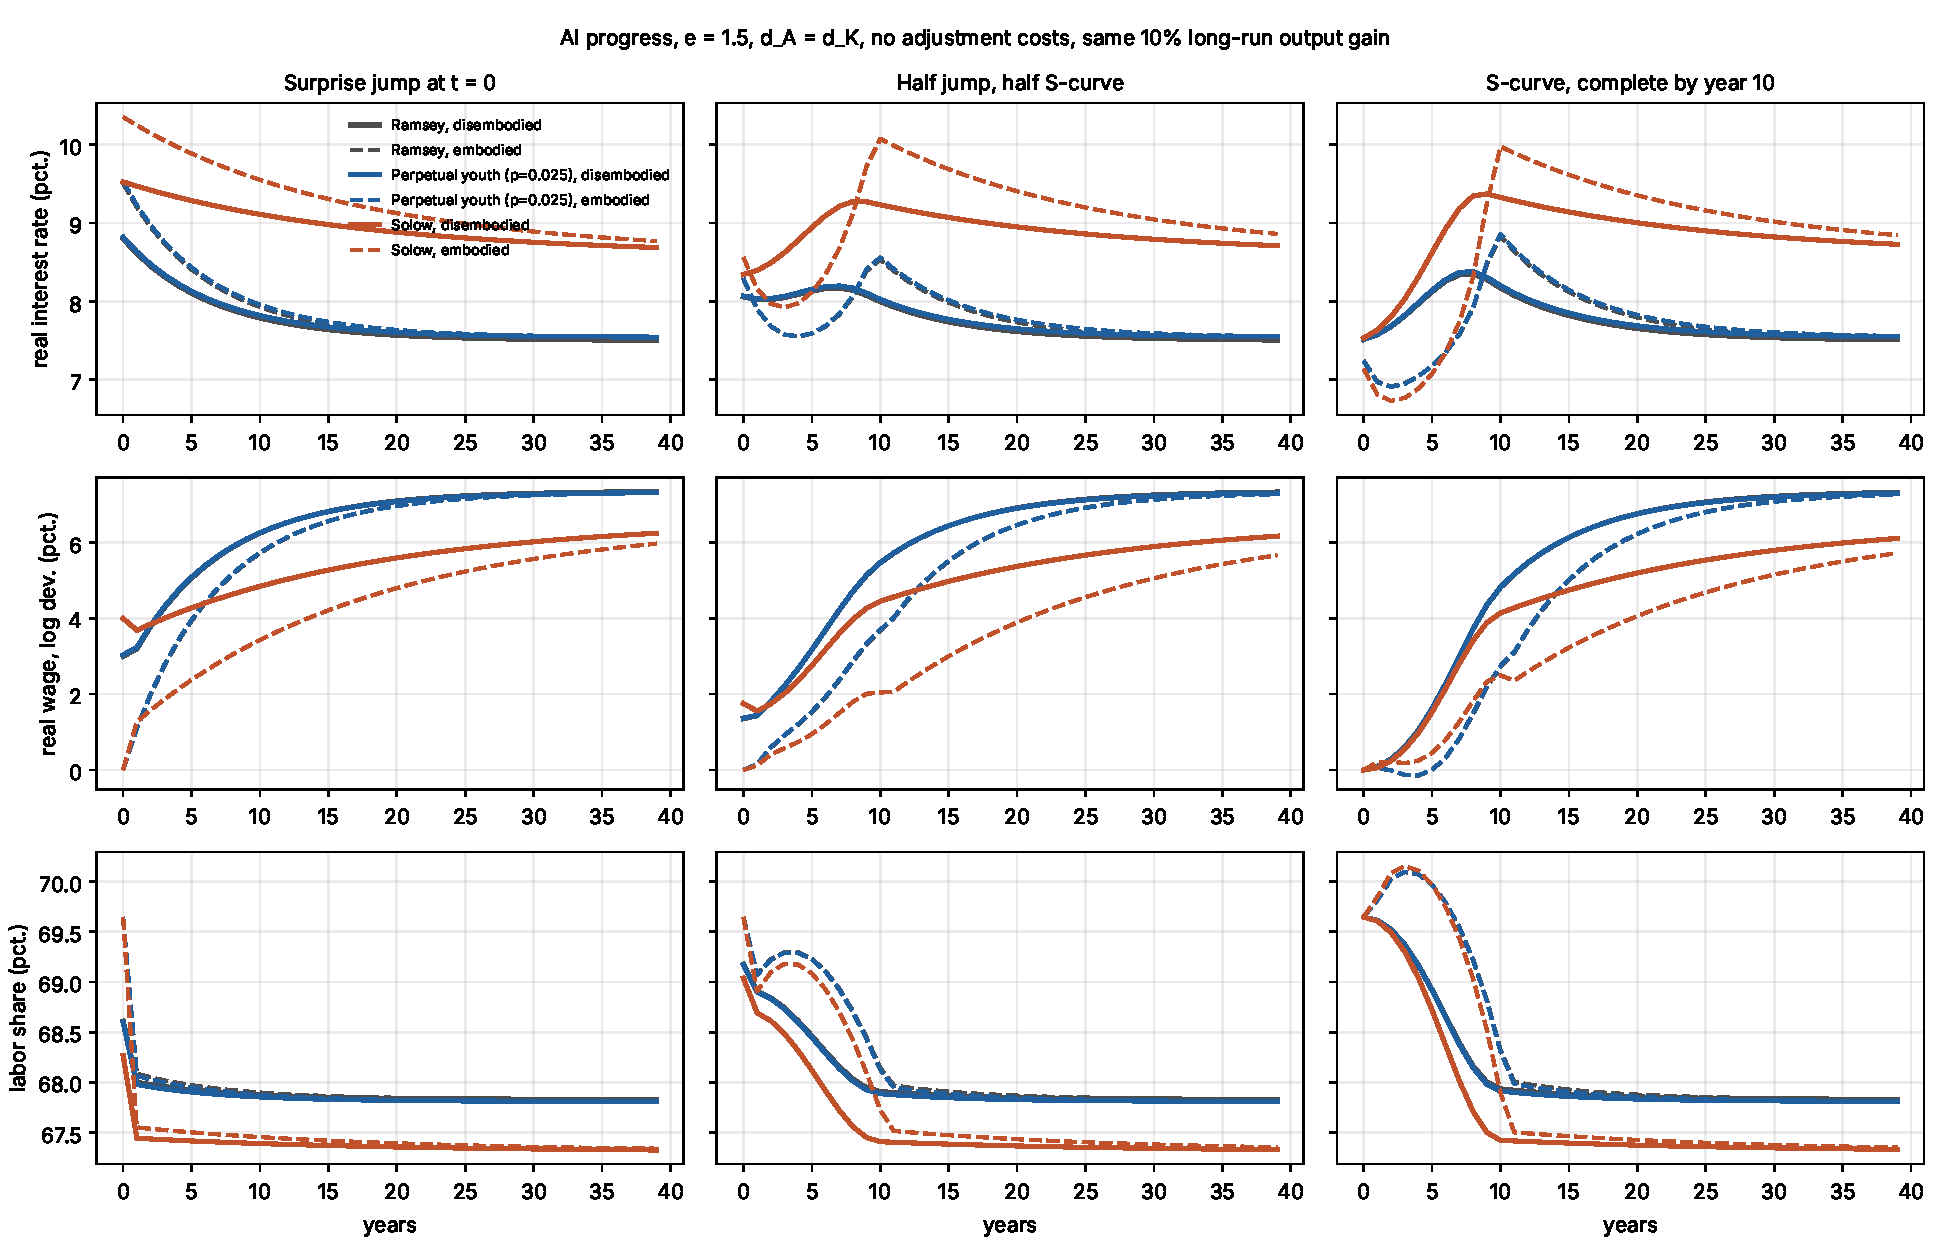
\includegraphics[width=\textwidth]{figures/fig_saving_trans_A.pdf}\\[4pt]
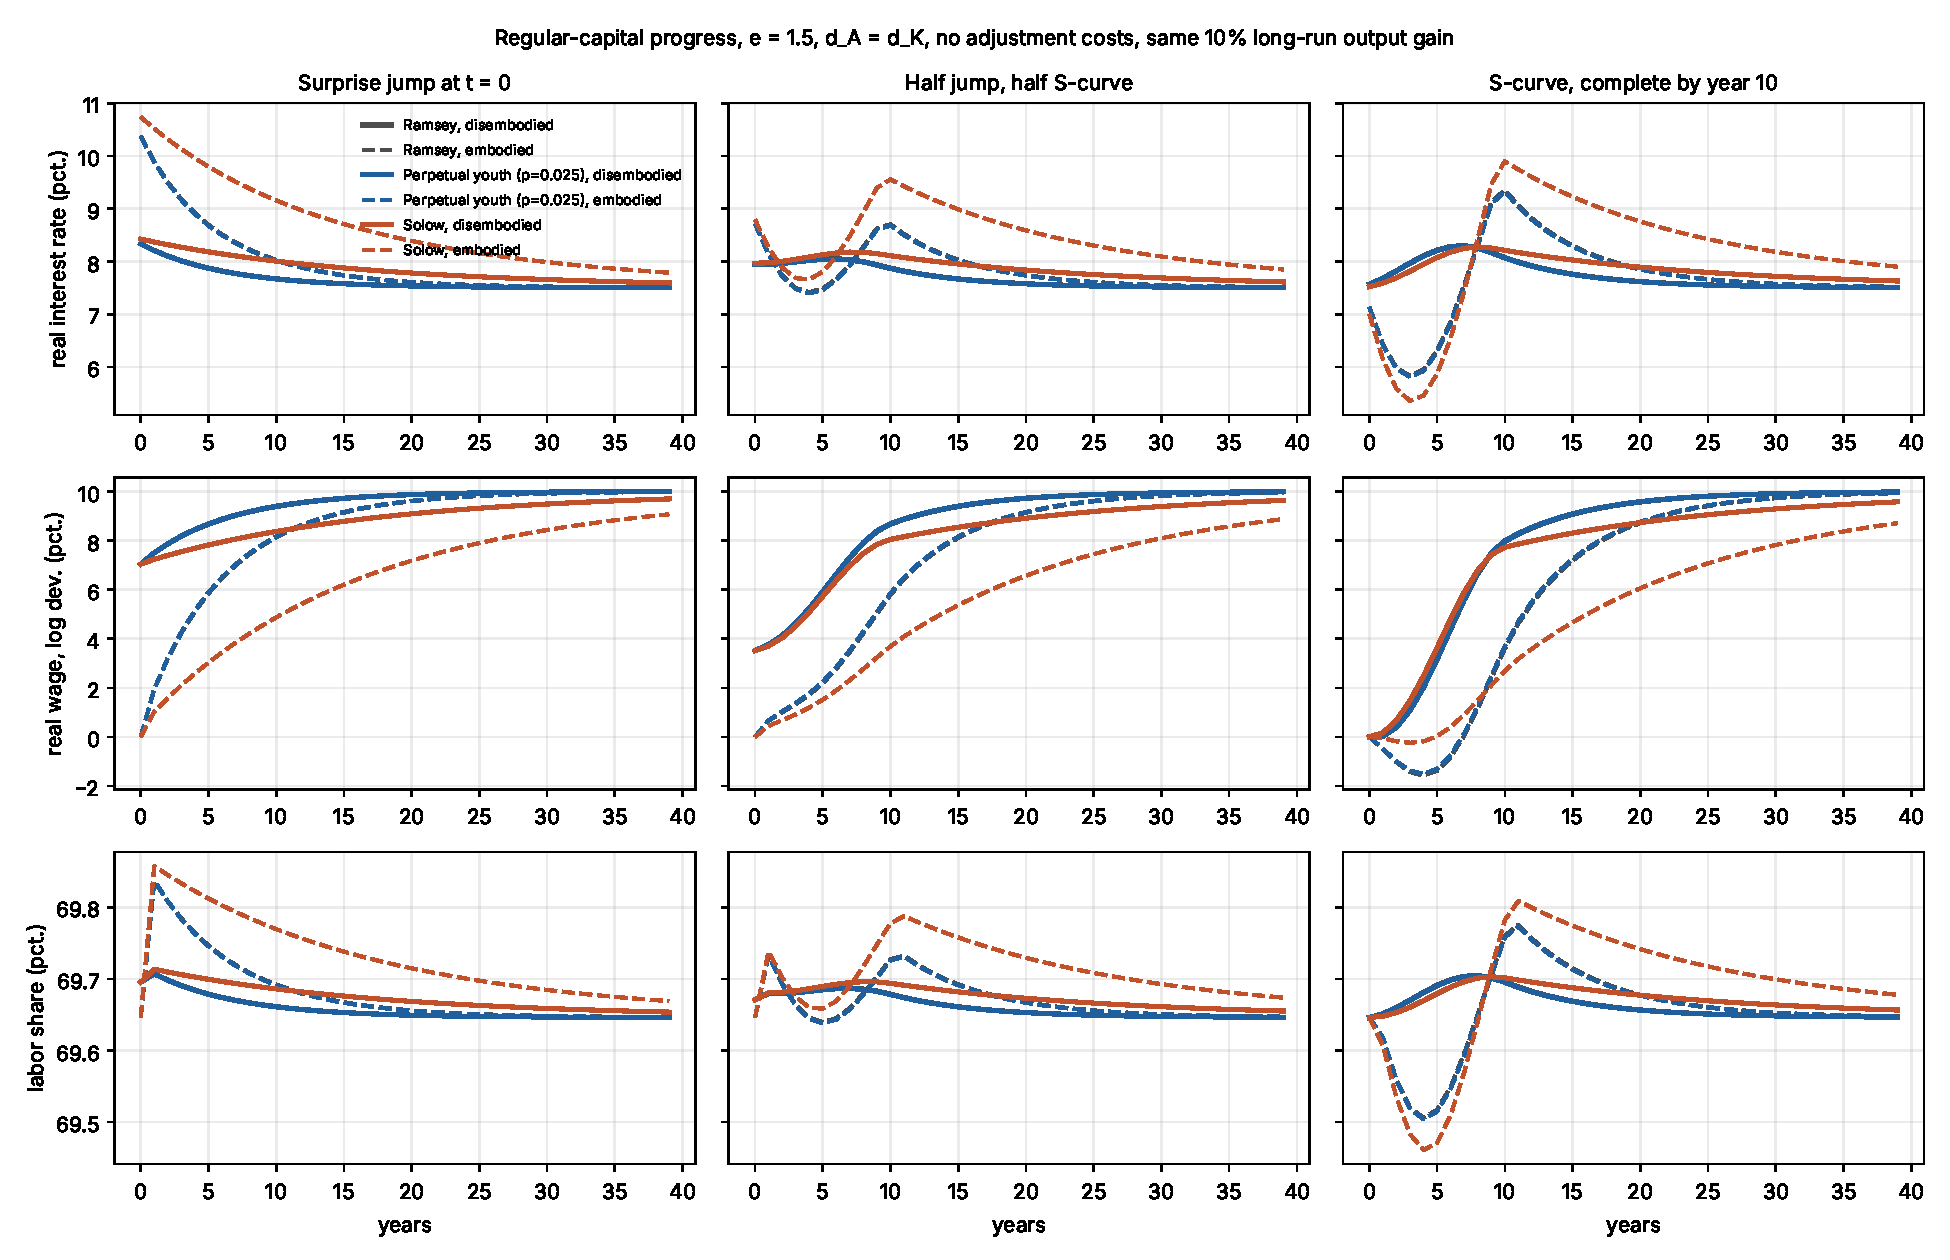
\includegraphics[width=\textwidth]{figures/fig_saving_trans_K.pdf}
\caption{Transitions by saving model, Setting B, $\e=1.5$. Top: AI progress. Bottom: regular-capital progress.}\label{fig:trans}
\end{figure}

\paragraph{Transitions (Figure~\ref{fig:trans}; full table in the appendix).}
\begin{itemize}
\item \emph{Perpetual youth and the annual OLG track Ramsey closely} (within about 0.1 point
for $r$), apart from the small permanent rise in $r$ after AI progress.
\item \emph{Solow amplifies and prolongs the AI response, and makes it permanent.} After
a jump, $r_1$ is 9.5 percent (disembodied) or 10.4 percent (embodied), against 8.8 and 9.5
under Ramsey. Along the S-curve it peaks at 9.4 (disembodied) or 10.0 (embodied), against
8.35 and 8.8. Then $r$ converges to 8.6 rather than 7.5 percent. Wages rise more slowly.
\item \emph{For regular-capital progress} the saving model matters only in the transition.
Solow gives larger embodied swings (S-curve trough 5.4 and peak 9.9 percent), and $r$
returns to 7.5 percent.
\item \emph{The embodied-anticipation dip in $r$} appears under every saving model.
\end{itemize}

\section{Summary}

\begin{enumerate}
\item With the same long-run output gain, AI progress raises wages by about three-quarters as much as
regular-capital progress and lowers the labor share. This holds in closed form, for
embodied and disembodied progress alike, and in every saving model. Less elastic saving
widens the gap.
\item Under Ramsey, the real-rate response depends mainly on whether progress is embodied and
on its timing: jumps versus anticipated S-curves, and the wait-for-cheaper-capital
dip. Substitutability matters only after surprise disembodied jumps.
\item The Ramsey result that substitutability barely moves $r$ comes from perfectly
elastic long-run capital supply. With fixed saving (Solow) or saving out of wages
(Diamond), AI progress with $\e>1$ raises long-run $r$ permanently, by up to 2 points at
$\e=2$. Regular-capital progress does not. Annual life-cycle (OLG) and perpetual-youth
saving are elastic enough that the effect is small, 0.1--0.2 points.
\end{enumerate}

\appendix
\section{Transitions by saving model}
\begin{table}[h]\centering\tiny
\caption{Transitions by saving model, Setting B, $\e=1.5$. ``Long run'' $r$ is the closed form of Proposition~\ref{prop:saving}.}
\begin{tabular}{lllcccccc}\toprule
 & & & \multicolumn{3}{c}{real rate (pct.)} & \multicolumn{2}{c}{$\ln W$ (pct.)} & labor share\\
\cmidrule(lr){4-6}\cmidrule(lr){7-8}
timing & progress & saving model & $r_1$ & max & long run & $t{=}10$ & long run & $t{=}10$\\\midrule
Jump & AI disemb. & Ramsey & 8.80 & 8.80 & 7.50 & 6.2 & 7.4 & 67.9\\
 &  & Perpetual youth & 8.82 & 8.82 & 7.54 & 6.3 & 7.3 & 67.9\\
 &  & Solow & 9.52 & 9.52 & 8.58 & 4.8 & 6.6 & 67.4\\
 & AI emb. & Ramsey & 9.51 & 9.51 & 7.50 & 5.7 & 7.4 & 67.9\\
 &  & Perpetual youth & 9.53 & 9.53 & 7.54 & 5.7 & 7.3 & 67.9\\
 &  & Solow & 10.35 & 10.35 & 8.58 & 3.4 & 6.6 & 67.5\\
 & Reg. disemb. & Ramsey & 8.33 & 8.33 & 7.50 & 9.4 & 10.0 & 69.7\\
 &  & Perpetual youth & 8.33 & 8.33 & 7.50 & 9.4 & 10.0 & 69.7\\
 &  & Solow & 8.42 & 8.42 & 7.50 & 8.4 & 10.0 & 69.7\\
 & Reg. emb. & Ramsey & 10.38 & 10.38 & 7.50 & 8.1 & 10.0 & 69.7\\
 &  & Perpetual youth & 10.37 & 10.37 & 7.50 & 8.2 & 10.0 & 69.7\\
 &  & Solow & 10.74 & 10.74 & 7.50 & 4.9 & 10.0 & 69.8\\
\midrule
Half/half & AI disemb. & Ramsey & 8.06 & 8.17 & 7.50 & 5.5 & 7.4 & 67.9\\
 &  & Perpetual youth & 8.07 & 8.20 & 7.54 & 5.5 & 7.3 & 67.9\\
 &  & Solow & 8.34 & 9.28 & 8.58 & 4.4 & 6.6 & 67.4\\
 & AI emb. & Ramsey & 8.29 & 8.53 & 7.50 & 3.7 & 7.4 & 68.1\\
 &  & Perpetual youth & 8.29 & 8.56 & 7.54 & 3.7 & 7.3 & 68.1\\
 &  & Solow & 8.56 & 10.07 & 8.58 & 2.0 & 6.6 & 67.7\\
 & Reg. disemb. & Ramsey & 7.95 & 8.05 & 7.50 & 8.7 & 10.0 & 69.7\\
 &  & Perpetual youth & 7.95 & 8.04 & 7.50 & 8.7 & 10.0 & 69.7\\
 &  & Solow & 7.97 & 8.18 & 7.50 & 8.0 & 10.0 & 69.7\\
 & Reg. emb. & Ramsey & 8.72 & 8.72 & 7.50 & 5.8 & 10.0 & 69.7\\
 &  & Perpetual youth & 8.71 & 8.71 & 7.50 & 5.9 & 10.0 & 69.7\\
 &  & Solow & 8.79 & 9.55 & 7.50 & 3.7 & 10.0 & 69.8\\
\midrule
S-curve & AI disemb. & Ramsey & 7.51 & 8.35 & 7.50 & 4.8 & 7.4 & 67.9\\
 &  & Perpetual youth & 7.51 & 8.38 & 7.54 & 4.8 & 7.3 & 67.9\\
 &  & Solow & 7.53 & 9.37 & 8.58 & 4.1 & 6.6 & 67.4\\
 & AI emb. & Ramsey & 7.24 & 8.83 & 7.50 & 2.7 & 7.4 & 68.3\\
 &  & Perpetual youth & 7.24 & 8.86 & 7.54 & 2.7 & 7.3 & 68.3\\
 &  & Solow & 7.14 & 9.97 & 8.58 & 2.5 & 6.6 & 67.9\\
 & Reg. disemb. & Ramsey & 7.57 & 8.30 & 7.50 & 8.0 & 10.0 & 69.7\\
 &  & Perpetual youth & 7.57 & 8.29 & 7.50 & 8.0 & 10.0 & 69.7\\
 &  & Solow & 7.52 & 8.28 & 7.50 & 7.7 & 10.0 & 69.7\\
 & Reg. emb. & Ramsey & 7.14 & 9.36 & 7.50 & 3.6 & 10.0 & 69.8\\
 &  & Perpetual youth & 7.13 & 9.33 & 7.50 & 3.7 & 10.0 & 69.8\\
 &  & Solow & 7.00 & 9.90 & 7.50 & 2.7 & 10.0 & 69.8\\
\bottomrule\end{tabular}

\end{table}

\section{Computation and verification}
All results are reproduced by \texttt{capital\_cases.py} (Settings A and B, run with the
\texttt{-{}-equal-d-noadj} switch) and \texttt{saving\_models.py} (saving models and the
elasticity grid). Each transition is a nonlinear perfect-foresight solve of the full
equilibrium.
\begin{itemize}
\item Ramsey, Solow and perpetual youth use Newton's method on the capital paths, with
residuals below $10^{-10}$.
\item The annual OLG uses Levenberg-Marquardt started from the Ramsey solution. Plain
Newton overshoots because life-cycle saving is very sensitive to returns. Residuals are
below $10^{-9}$. The OLG is solved over 300 years and its long run is read at year 200, because the final
cohorts carry a horizon-truncation artifact.
\end{itemize}
Further checks:
\begin{itemize}
\item Perpetual youth with $p=0$ reproduces the Euler-equation Ramsey solver.
\item Steady-state OLG household wealth equals the value of capital.
\item Every experiment converges to the 10 percent output gain and to the closed-form long-run $r$.
\item Long-run wages match Proposition~\ref{prop:lr}.
\end{itemize}

\begin{table}[h]\centering\tiny
\caption{Verification, saving models (largest errors).}
\begin{tabular}{lc}\toprule Check & max abs. error\\\midrule
ramsey e=0.75: initial r reproduces 7.5% & 0.0e+00\\
py e=0.75: initial r reproduces 7.5% & 6.9e-17\\
solow e=0.75: initial r reproduces 7.5% & 1.4e-17\\
diamond e=0.75: initial r reproduces 7.5% & 4.2e-17\\
ramsey e=1.0: initial r reproduces 7.5% & 0.0e+00\\
py e=1.0: initial r reproduces 7.5% & 6.9e-17\\
solow e=1.0: initial r reproduces 7.5% & 1.4e-17\\
diamond e=1.0: initial r reproduces 7.5% & 4.2e-17\\
ramsey e=1.5: initial r reproduces 7.5% & 0.0e+00\\
py e=1.5: initial r reproduces 7.5% & 6.9e-17\\
solow e=1.5: initial r reproduces 7.5% & 1.4e-17\\
diamond e=1.5: initial r reproduces 7.5% & 4.2e-17\\
ramsey e=2.0: initial r reproduces 7.5% & 0.0e+00\\
py e=2.0: initial r reproduces 7.5% & 6.9e-17\\
solow e=2.0: initial r reproduces 7.5% & 1.4e-17\\
diamond e=2.0: initial r reproduces 7.5% & 4.2e-17\\
ramsey jump K dis: residual & 2.4e-14\\
ramsey jump K dis: long-run ln Y = 10% & 9.3e-16\\
ramsey jump K emb: residual & 2.3e-15\\
ramsey jump K emb: long-run ln Y = 10% & 7.4e-16\\
ramsey jump A dis: residual & 2.7e-13\\
ramsey jump A dis: long-run ln Y = 10% & 7.4e-16\\
ramsey jump A emb: residual & 6.7e-14\\
ramsey jump A emb: long-run ln Y = 10% & 7.4e-16\\
ramsey mixed K dis: residual & 2.7e-15\\
ramsey mixed K dis: long-run ln Y = 10% & 9.3e-16\\
ramsey mixed K emb: residual & 9.8e-12\\
ramsey mixed K emb: long-run ln Y = 10% & 7.4e-16\\
ramsey mixed A dis: residual & 2.2e-15\\
ramsey mixed A dis: long-run ln Y = 10% & 7.4e-16\\
ramsey mixed A emb: residual & 1.0e-12\\
ramsey mixed A emb: long-run ln Y = 10% & 7.4e-16\\
ramsey scurve K dis: residual & 5.8e-14\\
ramsey scurve K dis: long-run ln Y = 10% & 9.3e-16\\
ramsey scurve K emb: residual & 2.4e-15\\
ramsey scurve K emb: long-run ln Y = 10% & 7.4e-16\\
ramsey scurve A dis: residual & 2.2e-15\\
ramsey scurve A dis: long-run ln Y = 10% & 7.4e-16\\
ramsey scurve A emb: residual & 2.0e-15\\
ramsey scurve A emb: long-run ln Y = 10% & 7.4e-16\\
py jump K dis: residual & 3.3e-14\\
py jump K dis: long-run ln Y = 10% & 3.3e-16\\
py jump K emb: residual & 3.7e-15\\
py jump K emb: long-run ln Y = 10% & 7.4e-16\\
py jump A dis: residual & 3.7e-13\\
py jump A dis: long-run ln Y = 10% & 3.3e-16\\
py jump A emb: residual & 9.7e-14\\
py jump A emb: long-run ln Y = 10% & 3.3e-16\\
py mixed K dis: residual & 2.1e-15\\
py mixed K dis: long-run ln Y = 10% & 3.3e-16\\
py mixed K emb: residual & 1.1e-11\\
py mixed K emb: long-run ln Y = 10% & 7.4e-16\\
py mixed A dis: residual & 2.0e-15\\
py mixed A dis: long-run ln Y = 10% & 3.3e-16\\
py mixed A emb: residual & 1.4e-12\\
py mixed A emb: long-run ln Y = 10% & 3.3e-16\\
py scurve K dis: residual & 6.3e-14\\
py scurve K dis: long-run ln Y = 10% & 7.4e-16\\
py scurve K emb: residual & 2.2e-15\\
py scurve K emb: long-run ln Y = 10% & 7.4e-16\\
py scurve A dis: residual & 2.4e-15\\
py scurve A dis: long-run ln Y = 10% & 3.3e-16\\
py scurve A emb: residual & 2.0e-15\\
py scurve A emb: long-run ln Y = 10% & 3.3e-16\\
solow jump K dis: residual & 9.0e-14\\
solow jump K dis: long-run ln Y = 10% & 1.8e-08\\
solow jump K emb: residual & 5.7e-15\\
solow jump K emb: long-run ln Y = 10% & 5.5e-08\\
solow jump A dis: residual & 3.5e-11\\
solow jump A dis: long-run ln Y = 10% & 3.2e-08\\
solow jump A emb: residual & 6.8e-11\\
solow jump A emb: long-run ln Y = 10% & 5.7e-08\\
solow mixed K dis: residual & 1.5e-13\\
solow mixed K dis: long-run ln Y = 10% & 2.2e-08\\
solow mixed K emb: residual & 2.1e-15\\
solow mixed K emb: long-run ln Y = 10% & 6.6e-08\\
solow mixed A dis: residual & 6.2e-15\\
solow mixed A dis: long-run ln Y = 10% & 3.9e-08\\
solow mixed A emb: residual & 1.6e-15\\
solow mixed A emb: long-run ln Y = 10% & 8.6e-08\\
solow scurve K dis: residual & 2.7e-13\\
solow scurve K dis: long-run ln Y = 10% & 2.5e-08\\
solow scurve K emb: residual & 2.0e-15\\
solow scurve K emb: long-run ln Y = 10% & 7.6e-08\\
solow scurve A dis: residual & 2.1e-15\\
solow scurve A dis: long-run ln Y = 10% & 4.5e-08\\
solow scurve A emb: residual & 2.6e-14\\
solow scurve A emb: long-run ln Y = 10% & 8.0e-08\\
Ramsey jump K dis: r1 = Euler-equation solver & 5.2e-14\\
Ramsey jump K emb: r1 = Euler-equation solver & 2.0e-13\\
Ramsey jump A dis: r1 = Euler-equation solver & 7.5e-15\\
Ramsey jump A emb: r1 = Euler-equation solver & 2.4e-11\\
Ramsey mixed K dis: r1 = Euler-equation solver & 4.0e-14\\
Ramsey mixed K emb: r1 = Euler-equation solver & 3.4e-13\\
Ramsey mixed A dis: r1 = Euler-equation solver & 8.0e-13\\
Ramsey mixed A emb: r1 = Euler-equation solver & 2.4e-14\\
Ramsey scurve K dis: r1 = Euler-equation solver & 2.8e-14\\
Ramsey scurve K emb: r1 = Euler-equation solver & 2.0e-15\\
Ramsey scurve A dis: r1 = Euler-equation solver & 8.0e-14\\
Ramsey scurve A emb: r1 = Euler-equation solver & 4.4e-15\\
\bottomrule\end{tabular}

\end{table}

\begin{thebibliography}{9}
\bibitem[Blanchard(1985)]{blanchard1985}
Blanchard, O.~J. (1985). ``Debt, Deficits, and Finite Horizons.'' \emph{Journal of Political Economy} 93(2): 223--247.
\bibitem[Diamond(1965)]{diamond1965}
Diamond, P.~A. (1965). ``National Debt in a Neoclassical Growth Model.'' \emph{American Economic Review} 55(5): 1126--1150.
\bibitem[Kiley(2000)]{kiley2000}
Kiley, M.~T. (2000). ``Stock Prices and Fundamentals in a Production Economy.''
FEDS Working Paper 2000-05, Federal Reserve Board.
\bibitem[Kiley(2004)]{kiley2004}
Kiley, M.~T. (2004). ``Stock Prices and Fundamentals: A Macroeconomic Perspective.''
\emph{Journal of Business} 77(4): 909--936.
\bibitem[Yaari(1965)]{yaari1965}
Yaari, M.~E. (1965). ``Uncertain Lifetime, Life Insurance, and the Theory of the Consumer.''
\emph{Review of Economic Studies} 32(2): 137--150.
\end{thebibliography}
\end{document}
